\documentclass[a4paper, 12pt]{article}

\usepackage{geometry}
\geometry{left=2cm, right=2cm, top=2cm, bottom=2cm}

\usepackage{cmap}
\usepackage{mathtext} 
\usepackage[T2A]{fontenc}
\usepackage[utf8]{inputenc}
\usepackage[english,russian]{babel}	

\usepackage{amsfonts,amssymb,amsthm,mathtools}
\usepackage{amsmath}
\usepackage{icomma} 

\usepackage{graphicx} 
\graphicspath{{picturies/}}
\usepackage{wrapfig}

\usepackage{array,tabularx,tabulary,booktabs}
\usepackage{longtable}
\usepackage{multirow}

\usepackage{caption}
\captionsetup{labelsep=period}

\renewcommand{\phi}{\varphi}
\newcommand{\eps}{\varepsilon}
\newcommand{\parag}[1]{\paragraph*{#1:}}

\newcounter{Points}
\setcounter{Points}{1}
\newcommand{\point}{\arabic{Points}. \addtocounter{Points}{1}}

\author{Радькин Кирилл, Б01-005}
\date{21.05.22}
\title{Лабораторная работа 4.1.2. Моделирование оптических приборов и определение их увеличения.}

\begin{document}
    \maketitle

    \textbf{\\В работе используются:} оптическая скамья, набор линз, экран, осветитель со шкалой, зрительная труба, диафрагма, линейка.

    \textbf{\\Теоретическая справка:}
        \begin{itemize}
            \item Формула для расчета фокусного расстояния рассеивающей линзы с помощью зрительной трубы
                \begin{equation}
                    \label{eq1}
                    f~=~l~-~a_0
                \end{equation}

            где $l$~---~расстояние между линзами, $a_0$~---~расстояние между собирающей (вспомогательной) линзы.

            \item Формула для расчета увеличения:
                \begin{equation}
                    \label{eq2}
                    N~=~\dfrac{\alpha'}{\alpha}~=~\dfrac{f_1}{f_2}~=~\dfrac{h_2}{h_1}
                \end{equation}

            где $f_1,~f_2$~---~фокусные расстояние соответствующих линз (зависит от установки), $h_1$~---~размер изображения одного миллиметра шкалы осветителя в делениях окулярной шкалы зрительной трубы, $h_2$~---~размер изображения миллиметрового деления шкалы осветителя в делениях окулярной шкалы трубы (после прохождения оптического прибора).

            \item Необходимый интервал $\Delta$(для микроскопа):
                \begin{equation}
                    \label{eq3}
                    N_M~=~N_1 \cdot N_2~=~\dfrac{\Delta}{f_1} \dfrac{L}{f_2} 
                \end{equation}

            где $f_1,~f_2$~---~фокусные расстояния соответствующих линз, $L~=~25$ см~---~расстояние наилучшего зрения, $N_M$~---~увеличение микроскопа.

            \item Длина тубуса микроскопа:
                \begin{equation}
                    \label{eq4}
                    l_{12}~=~\Delta + f_1 + f_2
                \end{equation}

            \item Увеличение микроскопа:
                \begin{equation}
                    \label{eq5}
                    N_M~=~\dfrac{h_2}{h_1} \dfrac{L}{f}
                \end{equation}
        \end{itemize}

    \textbf{\\Ход работы:}

    \begin{itemize}
        \item Центрировка элементов оптиеской системы
            \begin{enumerate}
                \item Определим, какие линзы из набора собирающие, а какие~---~рассеивающие. В нашем случае линзы $1, 2, 3, 4$~---~собирающие, линза $5$~---~рассеивающая. Оценим на глаз фокусные расстояния некоторых линз.\\
                
                    \begin{tabular}{|c|c|c|c|} \hline
                        Номер линзы & 1 & 2 & 3 \\ \hline
                        f, см & $8.0 \pm 0.1$ & $9.4 \pm 0.1$ & $16.0 \pm 0.1$ \\ \hline
                    \end{tabular}

                \item Центрируем систему
            \end{enumerate}

        \item Определение фокусных расстояний тонких линз с помощью зрительной трубы
            \begin{enumerate}
                \item Настроим трубу на бесконечность. Установим линзу на расстоянии от предмета примерно равном фокусному. Разместим трубу на небольшом расстоянии от линзы. Передвигая линзу вдоль скамьи, получим в окуляре трубы изображение, при этом расстояние между предметом и серединой тонкой линзы равно фокусному.
                
                \begin{figure}[!h]
                    \centering
                    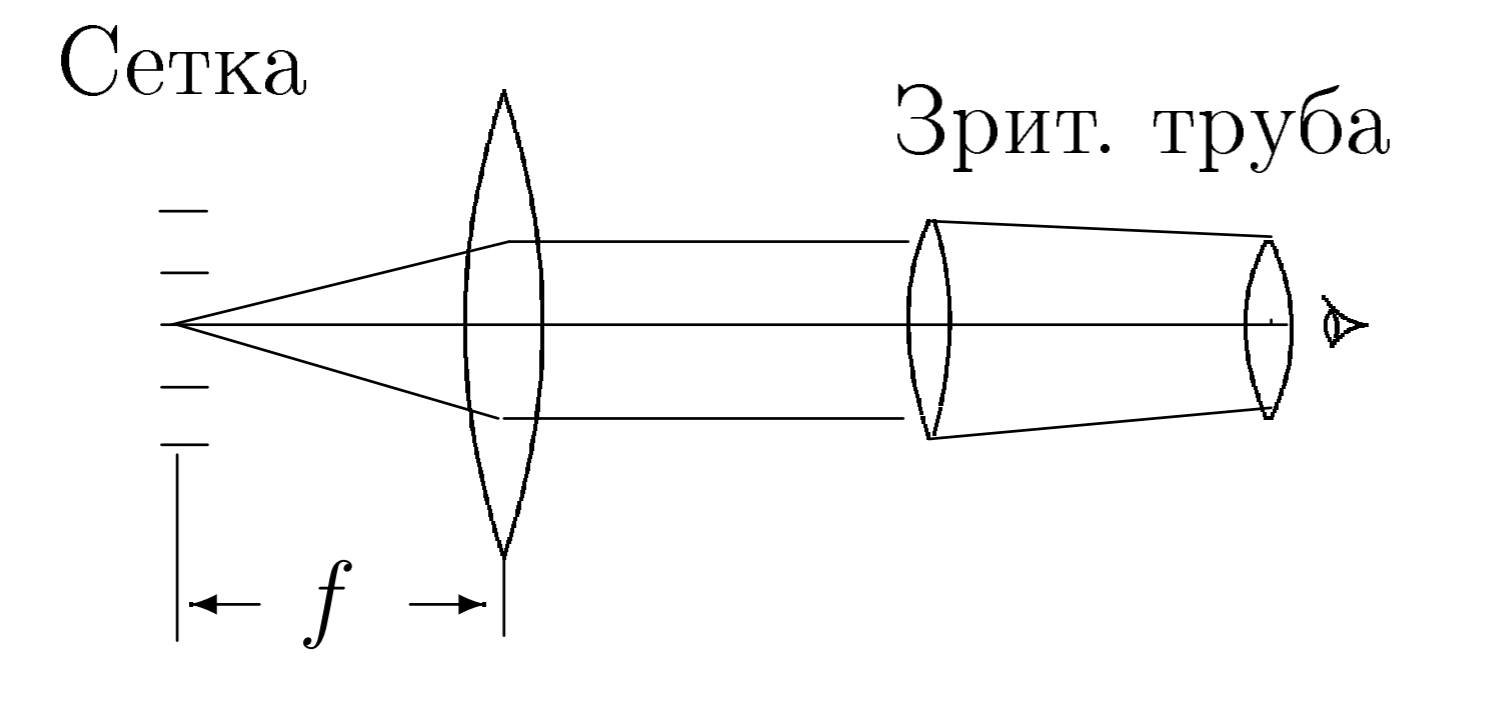
\includegraphics[scale = 0.3]{412-1.png}
                    \caption{Определение фокусного расстояние собирающей линзы}
                    \label{pic1}
                \end{figure}

                \item Запишем измеренные фокусные расстояния для собирающих линз\\
                
                    \begin{tabular}{|c|c|c|c|c|} \hline
                        Номер линзы & 1 & 2 & 3 & 4 \\ \hline
                        f, см & $7.5 \pm 0.5$ & $8.5 \pm 0.5$ & $16.0 \pm 0.5$ & $31.0 \pm 0.5$ \\ \hline
                    \end{tabular}

                \item Для определения фокусного расстояния рассеивающйе линзы сначала получим увеличенное изображение сетки с помощью одной короткофокусной лины ($f~=~8.5$ см). Измерим расстояние между линзой и экраном: $a_0~=40.5 \pm 0.5$ см. Разместим сразу за экраном трубу, уберем экран и, перемещая рассеивающую линзу, найдем в окуляре трубы изображение сетки. Измерим расстояние между линзами $l~=~36.0 \pm 0.5$ см. Таким образом получаем $f_5~=~-4.5 \pm 0.5$ см.
                
                \begin{figure}[!h]
                    \centering
                    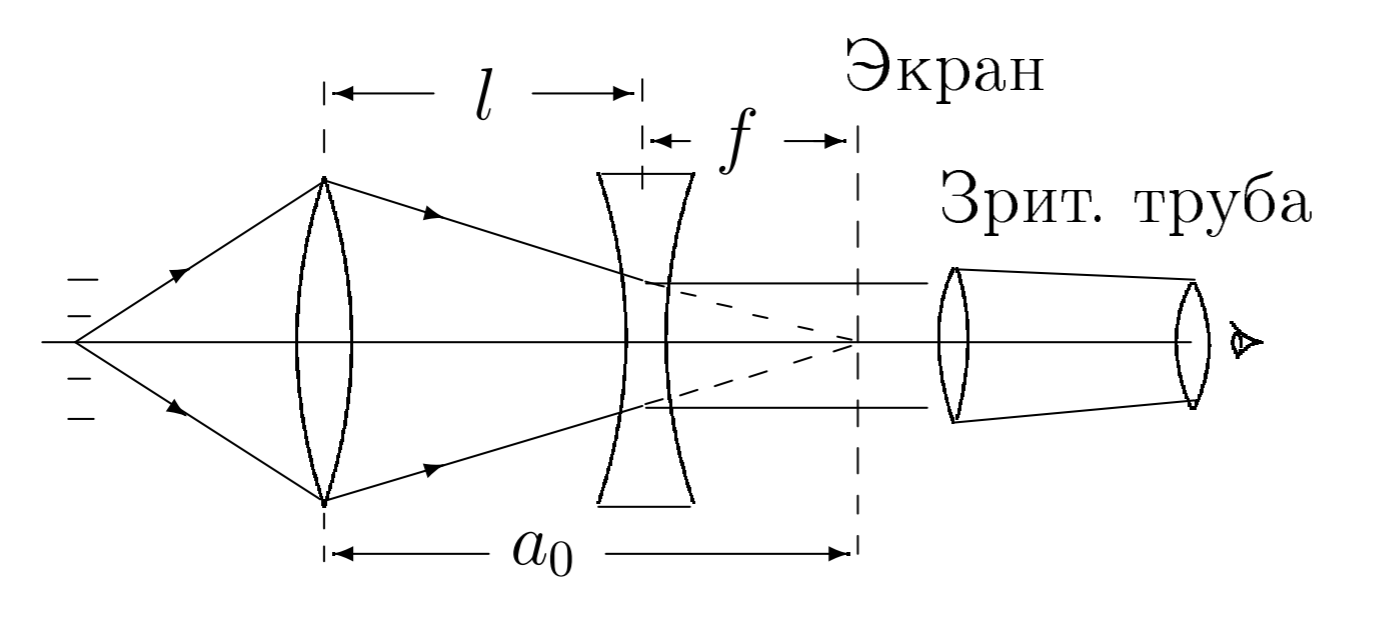
\includegraphics[scale = 0.4]{412-2.png}
                    \caption{Определение фокусного расстояние рассеивающей линзы}
                    \label{pic2}
                \end{figure}
            \end{enumerate}

        \item Телескоп Кеплера
            \begin{enumerate}
                \item Выберем две собирающие линзы (под номерами 2 и 1) для создания модели трубы Кеплера. В качестве коллиматора используем линзу 3.
                
                \begin{figure}[!h]
                    \centering
                    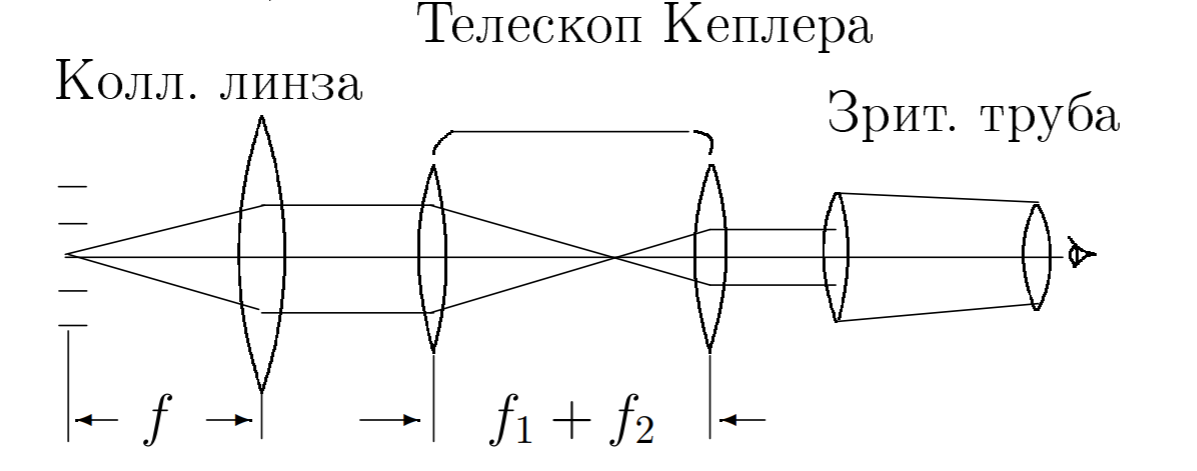
\includegraphics[scale = 0.5]{412-3.png}
                    \caption{Модель телескопа Кеплера}
                    \label{pic3}
                \end{figure}

                \item Определим размер изображения одного миллиметра шкалы осветителя в делениях окулярной шкалы зрительной трубы: $h_1~=~11$ см
                \item Соберем модель телескопа. Слегка перемещая окуляр модели, получим изображение миллиметровой сетки в окуляре трубы.
                \item Измерим расстояние между объективом и окуляром: $L~=~17 \pm 0.5$ см. Примерно совпадает с суммой фокусных расстояний ($16$ см).
                \item Рассчитаем увеличение полученной модели через отношение фокусных расстояний и через размер изображение (используя формулу \ref{eq2}), равный $h_2~=~15$ делений.  
                
                \begin{equation*}
                    N_Т~=~\dfrac{f_1}{f_2}~=~1.1 \pm 0.1
                \end{equation*}

                \begin{equation*}
                    N_T~=~\dfrac{h_1}{h_2}~=~1.5 \pm 0.2
                \end{equation*}
            \end{enumerate}

        \item Труба Галилея
            \begin{enumerate}
                \item Труба Галилея имеет такую же схему, как и телескоп Кеплера, только вместо собирающей окулярной линзы поставить рассеивающую на расстоянии от объектива, равном разности фокусов объектива и окуляра.
                \item Далее все измерения аналогичны телескопу Кеплера. $h_2~=~50$ дел.
                \begin{equation*}
                    N_Т~=~\dfrac{f_1}{f_2}~=~6.9 \pm 0.1
                \end{equation*}

                \begin{equation*}
                    N_T~=~\dfrac{h_1}{h_2}~=~4.6 \pm 0.2
                \end{equation*}
            \end{enumerate}

        \item Модель микроскопа
            \begin{enumerate}
                \item Для создания модели микроскопа используем линзы 1 и 2. Рассчитаем необходимый интервал и длину тубуса по формулам \ref{eq3} и \ref{eq4}. $\Delta~=~12.8 \pm 1.1$ см, $l_{12}~=~28.8 \pm 2.1$ см.
                \item Расположим объектив и окуляр на соответствующем расстоянии $l_{12}$ друг от друга. Сфокусируем модель микроскопа на сетку осветителя.
                \item Расположим за окуляром модели зрительную трубу, настроенную на бесконечность. Перемещая осветитель, получим изображение миллиметровой сетки.
                \item Измерим $h_2~=~35$ делений
                \item Используя результат аналогичных измерений с коллиматорной линзой, фоксное расстояние $f~=~16$ см известно, рассчитаем увеличение микроскопа по формуле \ref{eq5}: $N_M~=~4.9 \pm 0.1$
                \item Сравним его с теоретическим расчетом по формуле \ref{eq3}: $N_M = 5$
            \end{enumerate}
    \end{itemize}
\end{document}